\subsubsection{Opening a MySQL Database}
\label{sec:mysql_open_db}

After successful connection, all existing databases in the server are shown in the 'Database name' drop-down menu. The last used one is selected automatically.

\begin{figure}[H]
  \center
    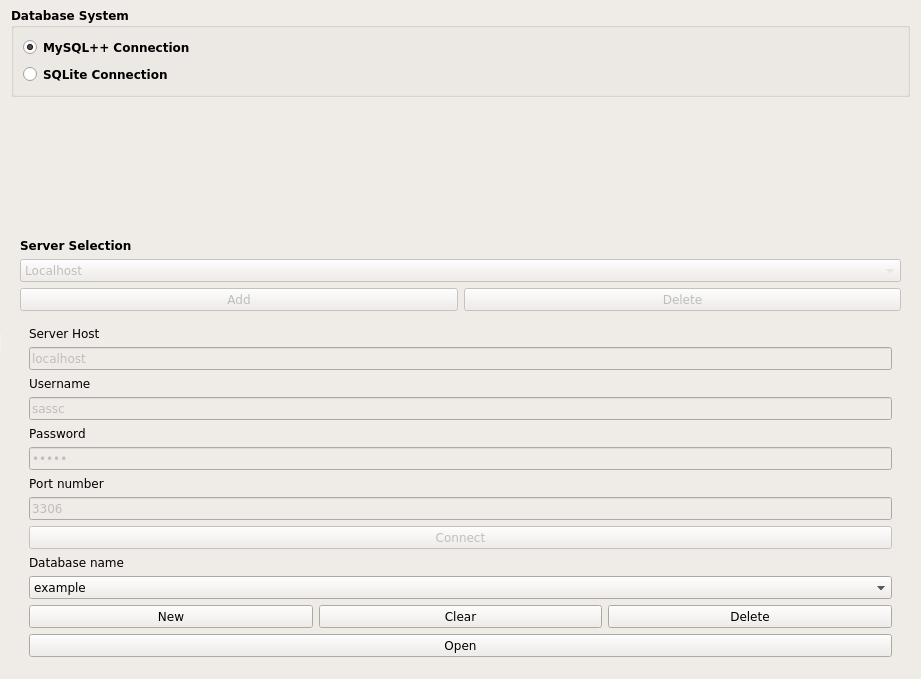
\includegraphics[width=5.5cm,frame]{../screenshots/mysql_database_selection.png}
  \caption{Selecting a MySQL database.}
  \label{fig:mysql_db_select}
\end{figure}

Several actions are available:

\begin{itemize}  
\item Drop-down selection: Selects the current database
\item New button: Allows creation of a new database
\item Clear button: Deletes all data with current database (after confirmation)
\item Delete button: Deletes current database (after confirmation)
\item Open button: Opens the current database
\end{itemize} 
